\section{The Simulated Data}
\subsection{Monte Carlo Simulated Data}
Up to this point in the thesis I have discussed two data sets: the measured collision data and the simulated \ac{MC} data. 
The simulated events are produced with software that relies on \acf{MC} techniques\footnote{For 
more information on \ac{MC} simulation, the reader is referred to \cite{raychaudhuri_introduction_2008}.}.
Through simulations, we are able to (among other things); test our understanding of the detector, model the expected \ac{SM} background 
events in different regions and model new \ac{BSM} physics. The pipeline for simulating collision events can be summarized in the following steps
\begin{itemize}
  \item \emph{Generate events}: Simulate each event in the collision, marking each event with the corresponding process (see section \ref{sec:bkg})
  \item \emph{Simulate detection of events}: Simulate the detection of each event in the different layers of the detector described in section \ref{subsec:Detector}
  \item \emph{Digitization}: Translate the interaction between the particles and the detector to a format that mimics exactly the digital signals from the detector
  \item \emph{Reconstruct events}: Apply the same software to the simulated digital signals that is applied to the real data, producing representations of physically 
              meaningful objects such as tracks, electrons, photons, jets and muons
\end{itemize}
I was not involved in the collection or production of either of the datasets, simulated or measured.
\subsection{The Simulated Signal}\label{subsec:signal}
As I have mentioned in previous sections I will be searching for a large range of signals, all related to the same
physics, but with different set of parameters, i.e. choices for the masses of the charginos and neutralinos. In figure \ref{fig:nrSignal} I have drawn a 
grid displaying the different mass combinations searched for in this analysis. The masses range from ${\tilde{\chi}_1}\in[0,400]$GeV
and ${\tilde{\chi}_2}\in[200,800]$GeV\footnote{The lightest chargino, $\tilde{\chi}^{\pm}_1$, and second neutralino, $\tilde{\chi}_2$, are mass degenerate, 
meaning they share the same mass. As a consequence, I will refer to the mass of each particle interchangeably throughout the thesis.}. In the beginning 
of my analysis I only received a subset (which will be referred to as the \emph{original} data set) of the full signal set. In figure \ref{fig:nrSignal} 
I have marked the original data set with a white label in the top right corner of the box. The original signal set contains a total of 30 different mass 
combinations in the ranges ${\tilde{\chi}_1}\in[0,400]$ and ${\tilde{\chi}_2}\in[400,800]$. In the full signal data set there are a total of 90 different 
mass combinations.
\\
Given that I received the original signal data set many months before receiving the full set, most of my results were carried out using the 
original set. Therefore, I chose to use the original data set to compare the performance of the models, then finally use the full set 
when comparing the results to previous analysis.
\begin{figure}
  \centering
  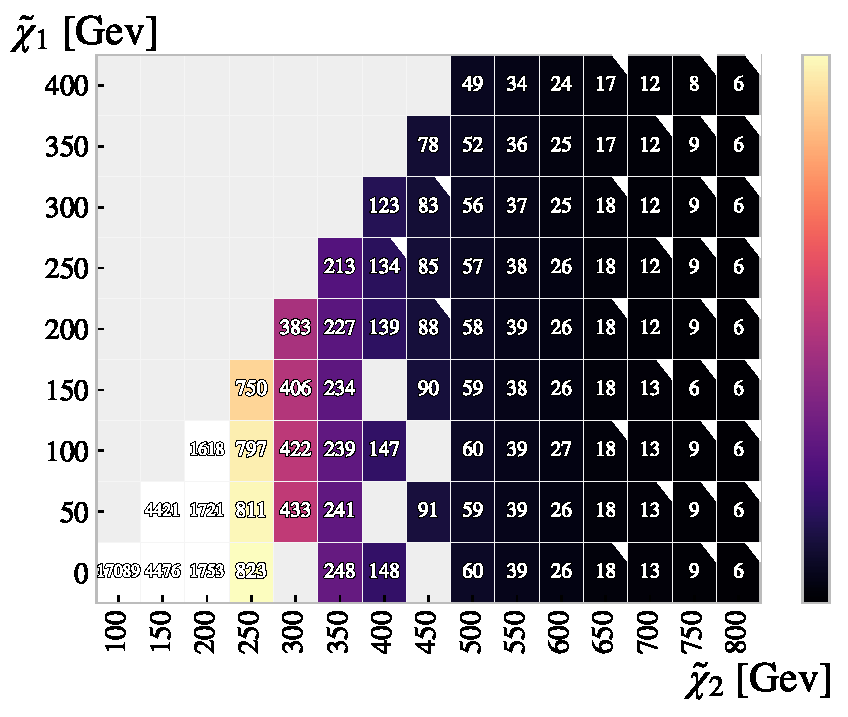
\includegraphics[width=0.85\textwidth]{Figures/MLResults/NN/SUSY/Grid/NrSignalEvents.pdf}
  \caption{A grid of all chargino and neutralino mass combinations and their respective event count in the full signal data set.
  Additionally, a white corner has been added to all combinations which define the original signal set.}
  \label{fig:nrSignal}
\end{figure}
\section{The Tools}
Every year technology for generating and measuring particle collisions is improving. 
As a consequence, the amount of data increases drastically. The \ac{ATLAS} experiment
is the largest particle detector experiment currently operating at the 
CERN laboratory near Geneva. \ac{ATLAS} alone generates approximately 60 terabyte of raw
data every second from proton-proton collisions at the \ac{LHC}. In this analysis I will 
be studying proton-proton collisions at a center of mass energy $\sqrt{s} = 13$TeV recorded by the \ac{ATLAS} detector 
between 2015-2018, corresponding to an integrated luminosity of $139.0fb^{-1}$. With amounts of data this large, 
data handling and storing is a big challenge. Therefore, taking advantage of sophisticated numerical tools 
and data frameworks is pivotal if scientific development is to keep up with technological development.
\subsection{ROOT}
In many aspects of my analysis, ranging from statistical analysis to plotting I utilize the \verb!ROOT! framework.
\verb!ROOT! \cite{ROOT} is at its core a large $\verb!C++!$ library and data structure made specifically for big data
analysis and computing, as well as data visualization. Today, all \ac{ATLAS} data is stored as \verb!ROOT! files, 
summing up to more than 1 exabyte ($10^{12}$) distributed globally via the Worldwide \ac{LHC} Computing Grid (WLCG)\cite{bird_update_2014}. 
\verb!ROOT! has many qualities which makes it ideal for particle physics analysis which demands heavy computations. Additionally, 
many particle physics-specific packages have been developed to make it an even better tool. Any function not already in library,
can easily be added in a \ac{HPC}-effective manner through $\verb!C++!$.
\\
Many of the plots presented in the present thesis were created using \verb!ROOT!. \verb!ROOT! has implemented a highly intuitive and
effective \ac{API} for data comparison and visualization, and allows for quick and direct 
comparison between data through an advanced graphical user interface. Furthermore, a lot of
functionality for creating complex stacked histograms are implemented in the \verb!ROOT! \ac{API}, such
as uncertainty calculations, ordering of histograms and statistical analysis tools. A final and important benefit of 
\verb!ROOT! is its impressive handling of memory and \acs{IO} which makes it ideal to handle large amounts of data.
\subsection{Data Structure and Frameworks}
Both data sets used as input to the analysis in this thesis, the measured and simulated, were stored in \verb!ROOT!, in the format of \verb!NTuples!. 
\verb!NTuples! are \verb!ROOT! objects designed to store large amounts of data. They allow for non-symmetrical entries, meaning 
cells with different number of entries. The simulated and measured collision data are both stored in \verb!NTuples!, with a matrix like structure 
where the columns represent the variables/features, and the rows represent each event. Hence, allowing ragged entries is essential 
for the purpose of storing data on particle collisions, given that the amount of information needed for each event can vary. For example the $p_T$ of the 
event from a three lepton final state would need three entries, whereas an event ending in a two lepton final state only needs two.
\\
When starting preprocessing I load the \verb!NTuples! using a \verb!ROOT! interface called \verb!RDataFrame!\footnote{For full 
documentation on RDataFrame, see \url{https://root.cern/doc/master/classROOT\_1\_1RDataFrame.html} 
(Accessed 16.04.2023).}. \verb!RDataFrame! allows for easy addition of new columns as well as filtering of events through native functionality. 
As a consequence I used \verb!RDataFrame! to calculate all features not already in the data set, such as the sum of transverse momentum, 
or the invariant mass of the three leptons. 
\\
After pre-processing was completed, I used \verb!RDataFrame!'s \emph{AsNumpy} function to translate the data frame into 
\verb!Numpy! objects \cite{numpy}, which then allowed me to transform it to a \verb!Pandas! data frame \cite{Pandas}. This is done
because \verb!Pandas!, like most \ac{ML}-tools, work in a strict \verb!Python! environment. \verb!Pandas!, similarly to \verb!RDataFrame!,
includes a deep computational library, and is optimal for analysis of big data. When the full \ac{ML} 
pipeline (data-handling, training, validation etc.) is completed the data is transformed back to \verb!NTuples!, 
to take advantage of the plotting functionality in \verb!ROOT!. The workflow of the data pre-processing is visualized in figure 
\ref{fig:WF}.
\begin{figure}
  \centering
  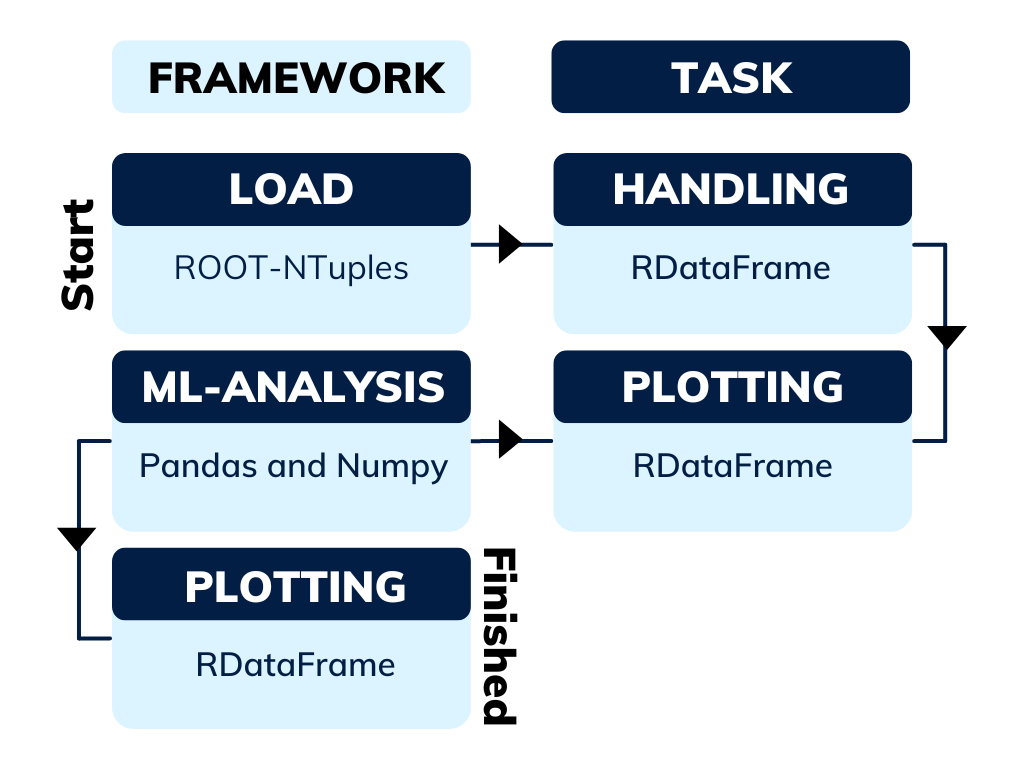
\includegraphics[width=0.6\textwidth]{Figures/Illustrations/TaskFlow.png}
  \vspace{-1cm}
  \caption{A visual summary of the workflow and frameworks used in the 
  computational analysis. }
  \label{fig:WF}
\end{figure}
\subsection{Computing Features in ROOT: Example}
In this section I will cover a simple example to highlight the steps taken in preparing the data set 
used in the analysis. As mentioned earlier, the two main frameworks used were \verb!RDataFrame! and \verb!Pandas!. 
In this example I will cover the case of a feature not already in the \verb!ROOT! file, namely the trilepton
invariant mass. All loading of data is done using the \verb!ROOT! framework and is easily read using the
\verb!RDataFrame! interface. To effectively generate new features I want to stay in \verb!ROOT! environment. Therefore,
I create a \verb!C++! file, \texttt{helperfunction}. The \texttt{helperfunction} contains additional 
\verb!ROOT! functions which are used in the analysis and are not already native to \verb!ROOT!. In the case 
of computing the trilepton invariant mass, the \verb!C++! function is created like shown in listing 
\ref{lst:mlll}.
\\
In listing \ref{lst:mlll}, we see a couple of measures taken to conform to the \verb!ROOT! environment. The first measure is 
the typecasting to $VecF\_t$. $VecF\_t$ is created to wrap floats in the native \verb!ROOT! vector object, $RVec$. 
The same is done in other cases such as float and integers, $VecI\_t$ and $VecB\_t$. The second measure
was using \verb!TLorentzVector! \footnote{For full documentation on TLorentzVector, see \url{https://root.cern.ch/doc/master/classTLorentzVector.html} (Accessed 16.04.2023).} 
to calculate the invariant mass. \verb!TLorentzVector! is a class native to \verb!ROOT! with many built-in functions. In 
this case we use the class to create four-vectors through the kinematic variables, $P_t$, $\eta$, $\phi$ and mass\footnote{These features
will be described in the next section \ref{sec:Feats}.}. Then, through the \verb!TLorentzVector! class we can simply add, through vector sums, 
together and extract the invariant mass of the three-lepton system. 
\lstset{style=Cpp}
\begin{lstlisting}[caption={$C{++}$-function which implementes the calculation of the trilepton invariant mass.},captionpos=b, label={lst:mlll}]
// Compute the trilepton invariant mass 
float ComputeInvariantMass(VecF_t& pt, VecF_t& eta, VecF_t& phi, VecF_t& m) {
  TLorentzVector p1;
  TLorentzVector p2;
  TLorentzVector p3;
  p1.SetPtEtaPhiM(pt[0], eta[0], phi[0], m[0]);
  p2.SetPtEtaPhiM(pt[1], eta[1], phi[1], m[1]);
  p3.SetPtEtaPhiM(pt[2], eta[2], phi[2], m[2]);
  return (p1 + p2 + p3).M();
}
\end{lstlisting}
The functions implemented in the \verb!C++! library (\texttt{helperfunction}) off-loads, from \verb!Python!, all the time, passing work to \verb!C++!,
which significantly speeds up the computation. The \verb!C++! library is compiled prior to the execution of the main \verb!Python!-code, which 
will be presented in the following. The main code, doing the selections, calculations and plotting, uses the \verb!RDataFrame! interface in a \verb!Python! 
environment. Whenever heavy calculations are needed the \verb!RDataFrame! interface calls on function in the \verb!C++! library described above. 
\\
In the code written in listing \ref{lst:df_mlll}, I show a simple example 
of loading new \verb!C++! functions, filtering out events, calculating new features and adding said 
features to a histogram. The first three lines of code both compiles and include the \texttt{helperfunction} 
into the \verb!ROOT! framework. Then I loop over all keys in the data frame, which in my case
are the different channels (i.e diboson, $t\bar{t}$ etc.). For each channel I select 'good' events,
based on the criteria I will present in section \ref{subsec:Cuts}. Then I use \verb!RDataFrame!'s \texttt{Define} function to calculate
and add a new feature using the \texttt{ComputeInvariantMass}-function. Finally, I save the feature as \verb!ROOT! object called 
\texttt{Histo1D}, which I later plot using \verb!ROOT! \ac{API}. In this example I chose the trilepton invariant mass, 
but in the analysis all additional features were calculated using a similar method. 
\lstset{style=Python}
\begin{lstlisting}[caption={Python-file for calling dataframe and calculating the trilepton invariant mass.},captionpos=b, label={lst:df_mlll}]
R.gROOT.ProcessLine(".L helperFunctions.cxx+");
R.gInterpreter.Declare('#include "helperFunctions.h"') 
R.gSystem.Load("helperFunctions_cxx.so")

for k in df.keys():
    # Define good leptons
    isGoodLepton = "feature1 < cut1 && feature2 >= cut2"

    # Define good leptons in dataframe
    df[k] = df[k].Define("isGoodLepton",isGoodLepton)

    # Define number of good leptons
    df[k] = df[k].Define("nGoodLeptons","ROOT::VecOps::Sum(isGoodLepton)")

    # Demand 3 good leptons 
    df[k] = df[k].Filter("nGoodLeptons == 3")

    # Define Invariant Mass (lll)
    df[k] = df[k].Define("mlll","ComputeInvariantMass(lepPt[isGoodLepton], 
                                                      lepEta[isGoodLepton], 
                                                      lepPhi[isGoodLepton], 
                                                      lepM[isGoodLepton])")
    # Add to histogram
    histo["mlll_%s"%k] = df[k].Histo1D(("mlll_%s"%k,
                                        "mlll_%s"%k,40,50,500),
                                        "mlll",
                                        "wgt_SG")     
\end{lstlisting}



